\documentclass[10pt,letter]{article}
\usepackage{amsmath}
\usepackage{amssymb}
\usepackage{graphicx}
\usepackage{setspace}
\usepackage{stmaryrd}
\def\fatbar{\talloblong}
\onehalfspacing
\usepackage{fullpage}
\newcommand{\R}{\mathbb{R}}	
\newcommand{\inner}{\langle\cdot,\cdot\rangle}
\newcommand{\inr}[2]{\langle #1, #2\rangle}
\newcommand\norm[1]{\left\lVert#1\right\rVert}

\graphicspath{ {images/} }

\begin{document}


\title{CS142 Homework Set \#5 Solutions}

\author{Timur Kuzhagaliyev}

%\date{7th November, 2017}
 
\maketitle 

\section*{Problem 1}

\paragraph{a)} I'll use an algorithm based on a concept of a diffusing computation similar to gossip algorithm in Sivilotti 6.5, modified to pass the total number of children $+ 1$ to the parent. I'll use the same specification and definitions as in Sivilotti 6.4, with 2 changes. I will adjust the definitions of $msg(x, y)$ and $done$ to fit our problem:
\begin{align*}
msg(x, y)\quad \equiv \quad &\textrm{tuple value $(p, c)$ of the message in the channel from $x$ to $y$,}
\\
& \textrm{where $p$ is the parent of the sender (if any) and $v$ is some integer}
\\
done\quad \equiv \quad &(\; \forall\; v : v\; nbr\; I : msg(v, I) \land (msg(v, I).p = I \Rightarrow  msg(v, I).c = -1)\;\; )
\end{align*}

Note about notation: When $msg(x, y)$ is used on its own (without accessing the values in the tuple), its interpreted as "there is a message in channel from x to y".

First, we define a UNITY program for the agent $I$ that initiates the diffusing computation. Its task is to send the initial gossip messages to all of its neigbours. Once it gets a message back, it checks that it's the parent of the sender and increments the vertex count by the reported value.
\begin{align*}
\textrm{\textbf{Program}} \qquad & \textrm{Initiator}\; I
\\
\textrm{\textbf{var}} \qquad & vertex\_count\; \textrm{:\; int}
\\ & msg(a, b)\; \textrm{:\; channel from $a$ to $b$}
\\
\textrm{\textbf{initially}} \qquad & vertex\_count = 1
\\
\land\; & (\; \forall\; v : v\; nbr\; I : \neg\, msg(v, I) \land \neg\, msg(I, v)\; )
\\
\textrm{\textbf{assign}} \qquad &
(\, \fatbar\, v : v\; nbr\; I : \neg\, msg(I, v) \longrightarrow msg(I, v) := (-1, -1)\; )
\\
\fatbar\quad & (\, \fatbar\, v : v\; nbr\; I : msg(v, I) \land msg(v, I).p = I \land msg(v, I).c \neq -1 \longrightarrow 
\\
& \qquad \qquad vertex\_count,\; msg(v, I).c := vertex\_count + msg(v, I).c,\; -1\; )
\end{align*}

I will refer to actions as $I1$ and $I2$. The action $I2$ of program \texttt{Initiator} checks whether $I$ is the parent of the incoming message. If it is, it adds the count passed in the message to $vertex\_count$ and resets the value in the message to $-1$. If the value in the message is already $-1$, it is ignored. By definition of $done$, $done$ will hold when $I$ has received a message from each of its neighbours and processed them using the logic I just described.

Now we define a UNITY program for all other agents which will be spreading the gossip. It's a modified version of the Gossip program in Sivilotti 6.5. The middle action executes the same logic as described in the paragraph above, but applied to \texttt{Gossip} program instead.
\begin{align*}
\textrm{\textbf{Program}} \qquad & \textrm{Gossip}\; u
\\
\textrm{\textbf{var}} \qquad & vertex\_count_u\; \textrm{:\; int}
\\ & parent_u\; \textrm{:\; process}
\\ & state_u\; \textrm{:\;} \{idle, active, complete\}
\\ & msg(a, b)\; \textrm{:\; channel from $a$ to $b$}
\\
\textrm{\textbf{initially}} \qquad & vertex\_count = 1
\\
\land\; & state_u = idle
\\
\land\; & (\; \forall\; v : v\; nbr\; u : \neg\, msg(u, v)\; )
\\
\textrm{\textbf{assign}} \qquad &
(\, \fatbar\, v : v\; nbr\; u : state_u = idle \land msg(v, u) \longrightarrow
\\
& \qquad \qquad parent_u := v\; 
\\
& \qquad \qquad \lVert\;\; state_u := active\;
\\
& \qquad \qquad \lVert\;\; (\; \forall\; w : w\; nbr\; u \land w \neq v : msg(u, w) := (v, -1)\; ) )
\\ &
\fatbar (\, \fatbar\, v : v\; nbr\; u : state_u = active \land msg(v, u) \land msg(v, u).p = u \land msg(v, u).c \neq -1 \longrightarrow
\\
& \qquad \qquad vertex\_count_u,\; msg(v, u).c := vertex\_count + msg(v, u).c,\; -1\; )
\\ &
\fatbar state_u = active \land (\, \forall\, v : v\; nbr\; u \land v \neq parent_u : msg(v, u) \land (msg(v, u).p = u \Rightarrow  msg(v, u).c = -1)\;) \longrightarrow
\\
& \qquad \qquad msg(u, parent_u) := (parent_u,\, vertex\_count_u)\; 
\\
& \qquad \qquad \lVert\;\; state_u := complete\;
\end{align*}

I will refer to the actions as $A1$, $A2$ and $A3$ respectively. The action $A3$ in my definition of \texttt{Gossip} is similar to that in Sivilotti 6.5, except I also check that for all incoming messages which defined $u$ as their parent the count $c$ is set to $-1$. That is, I make sure that all relevant counts were added to $vertex\_count_u$ before reporting it to the parent process.

Note that both \texttt{Initiator} and \texttt{Gossip} programs start out with $vertex\_count$ equal to $1$ because they automatically count themselves as a vertex.

\paragraph{b)} The proof for termination of diffusing computations can be found in Sivilotti 6.6. My algorithm is a modified version of the gossip algorithm Sivilotti uses.

\paragraph{c)} To prove that $I.vertex\_count$ has the correct counts at termination, we can define and prove another safety property: $\textrm{\textbf{invariant}} (done \Rightarrow I.vertex\_count = C)$ where $C$ is the true vertex count in the graph.

To prove that this new safety property holds I will extend the proof given in Sivilotti 6.6. There, he defines $T_1$ and $T_2$, proving the invariant that both are trees. We also know that the diffusing computation terminates, so eventually the "gossip" reaches all of the vertices, and each vertex eventually receives counts from its children and reports its count to its parent. Similar to Sivilotti 6.6.1, action $A3$ can delete a vertex from $T_2$, and it can be shown by contradiction that the deleted vertex must be a leaf in $T_2$.

We can show that when $T_2$ shrinks back to the state where it just contains $I$, $I.vertex\_count$ will be the correct count, by considering subtrees of $T_2$, when $T_2$ has all of the vertices from the original graph (i.e. right before it begins to shrink).

We know that $done$ will only hold after $I$ has received messages from all of its neighbours and action $I2$ has been executed on every incoming message, for which $I$ is the parent of the sender. This means $I$ would have taken the counts from these messages and added them to its $vertex\_count$. Since $vertex\_count$ starts out as $1$, after $done$ holds $I$ will hold the correct counts given that each child of $I$ in $T_2$ has reported the correct counts for the subtree this child is a root of.

We can show that the same condition applies to all vertices in $T_2$ that are a root of some subtree of $T_2$, apart from leaf vertices of $T_2$. This is true because action $A3$ only sends out a message once it received a message from all of its non-parent neighbours and the messages have been processed, that is $A_2$ has been applied to all incoming messages for which the current vertex is the parent of the sender. Again, if all children have reported the correct counts, the root of the subtree will have the correct $vertex\_count_u$ and report it to its parent.

Finally, the leaf vertices in $T_2$ would have no children by definition of $T_2$ - if they would have children they would not be leaves when $T_2$ contains all vertices from the original graph. This means that action $A2$ will never run and will never increment $vertex\_count_u$, so its value will just remain $1$. If the leaf has no other neighbours but the parent, it will simply report $1$ to the parent, which is the correct count since the subtree only has 1 vertex. If the leaf node has other neighbours, we know that a diffusing computation eventually reaches all vertices, so eventually current vertex will receive a message from all of its non-parent neighbours and finally report $1$ to its parent.

From 3 points above we can conclude that $I.vertex\_count$ would have the correct counts since each of its children would report the counts of its respective subtrees, and these counts will be correct given every subtree under a particular child reports the correct counts. The base case is a leaf node, and we've shown that a leaf node would report a correct count of $1$. Building up, this shows that every subtree would report the correct count, hence $I$ would receive the correct counts from its children.

\section*{Problem 2}

\paragraph{a)} To show that the provided property is required, let's consider a modified version of Lamport's mutual exclusion algorithm where the agent just needs to receive a message from every other agent after sending the request, but the logical time on these messages need not be larger than requested access time $t_i$. We will show that this modified version does not satisfy the safety property.

Consider the execution path where processes $P_1$ and $P_2$ have already communicated before, and $P_1$ has successfully entered the critical section (CS). In the beginning of timeline below, $P_1$ is just about to leave the CS and notify $P_2$ about it. As you can see at logical time $7$ on $P_2$, its queue still contains that older request from $P_1$.

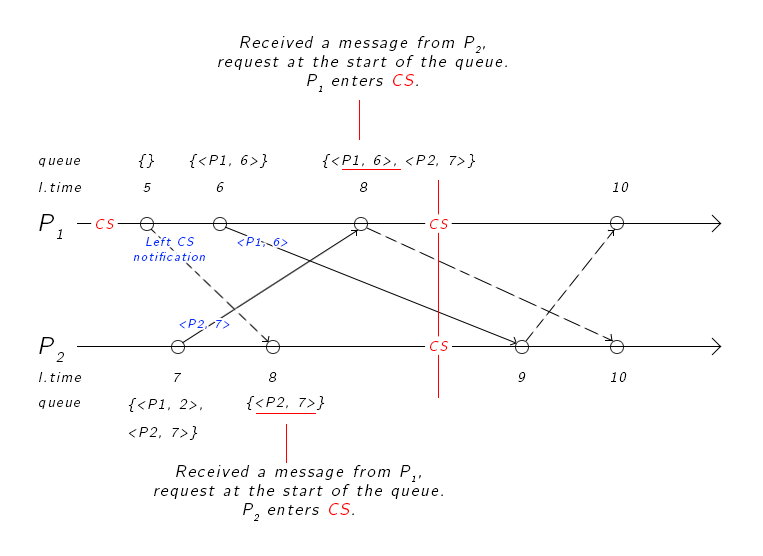
\includegraphics[width=\textwidth,height=\textheight,keepaspectratio]{hw5_problem2}

\paragraph{Explaining the diagram:} At time $7$ $P_2$ sends out a message requesting access to the critical section. At time $8$, it receives a message from $P_1$ saying that it has left the critical section. In our modified version of Lamport's algorithm, even though the timestamp on the message from $P_1$ is $5$ and hence smaller than local logical time, we still treat it as an $ACK$ and enter the critical section.

Process $P_1$ sends out its own request for access at local time $6$, and waits for any messages from $P_2$. At local time $8$, it receives a request $<P2, 7>$ from $P_2$, but the time of the request is larger than $P_1$'s own request. $P_2$'s request goes to the end of the queue. Now, $P_1$ has received a message from $P_2$ and its request is in the head of the queue - hence it enters the CS, by our modified version of Lamport's algorithm.

Now we have 2 processes in the critical section at the same time, so using \textit{any} messages as ACKs instead of messages with larger logical clock value is not sufficient.

\pagebreak

\paragraph{b)} Consider the following timeline:

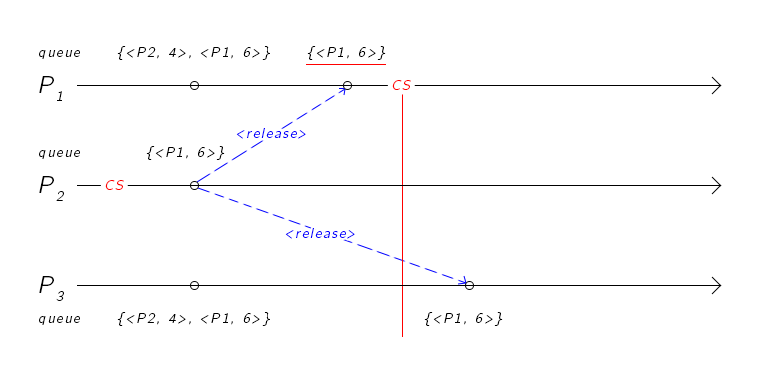
\includegraphics[width=\textwidth,height=\textheight,keepaspectratio]{hw5_problem2_b}

At the beginning of the timeline, we assume that all processes have already communicated before. $P_2$ is in the CS, $P_1$ is waiting for $P_2$ to leave the CS and $P_3$ simply maintains a queue without requesting access to CS. Once $P_2$ exits CS, it broadcasts a release message which gets delivered to $P_1$ sooner than to $P_3$. Since $P_1$'s request is now at the head of the queue and its request timestamp is smaller than all known times, it will now enter the CS. This can happen before $P_3$ will receive the release message, so $P_1$ will be in CS without being at the head of the queue for all agents.
\\

This cannot happen when there are no messages in transit. By definition of Lamport's algorithm, if there are no messages in transit, either all agents are in the non-critical section (NC) of code or there is a single agent that is currently inside CS with zero or more agents waiting for it to exit the CS. In the first case, since all agents are in NC, there is no reason for them to communicate so there are no messages in transit. In the second case, all agents have already exchanged requests and ACKs, and now are just waiting for the agent inside CS to exit and notify all other agents so next process can enter it.

We're interested in the second case. Let's denote the process that's currently in CS as $P_{CS}$. $P_{CS}$ could've entered CS by either being the first process to request access and receive ACKs from all other agents OR by being the second process in the queue and popping the head of the queue after the previous process exits CS.

We know that there are no requests with timestamps lower than $P_{CS}$'s request because all messages were already delivered and there are no messages in transit. If $P_{CS}$ was the very first process to request access, by now it would have received ACKs from all other agents and will now be in CS. At the same time, we know that it's at the head of every other agent's queue because it has the smallest request time and all messages have been delivered.

If $P_{CS}$ was the second (earliest) process to request access and have now popped the head of the queue to become first, it must have received a release message from the previous process in CS. Since no messages are in transit, all other processes would have also received the same notification and popped the previous process of their queues. Now, $P_{CS}$ has the smallest request time and all other agents have $P_{CS}$'s request on their queue since all messages were delivered. This means $P_{CS}$ is at the head of the queue for every agent when it enters CS.

Therefore, if there are no messages in transit and $P_{CS}$ is inside the CS, $P_{CS}$'s request must be at the head of queue for all agents.

\section*{Problem 3}

Description of the problem suggests that the algorithm does not involve agents sending ACKs back when they receive a request, so I will assume that this is indeed the case. Also assuming there is only one FIFO channel (in each direction) between any 2 agents.

The question doesn't bound the value of $\tau$ above, so I will assume that $\tau$ is finite, i.e. \texttt{my-time} will be broadcast eventually. The question also suggests that no release or request messages are sent at time $n*\tau$ - I will assume that request and release messages are timestamped with the time at which they have been sent, and not at the time they have been queued. That is, if the request message was about to be sent but it was time to broadcast \texttt{my-time}, the timestamp on the request message once its sent will be larger than reported \texttt{my-time}.

\paragraph{Proving safety:} We need to show that multiple agents cannot be in CS at the same time. We can prove that this is the case by contradiction.

Assume we have 2 agents, $P_1$ and $P_2$ in CS at the same time. For this to be true, their corresponding request times $z_1$ and $z_2$ must be the smallest timestamps in their lists $L$.

Assume, wlog, that $z_1 < z_2$. For $P_2$ to be in CS, it must be true that $z_2 < \textrm{REMOTE\_TIMES}[P_1]$. Since message channels are FIFO and $\textrm{REMOTE\_TIMES}$ is updated on any received message, $P_1$'s request must be in $P_2$'s list $L$, and hence $P_2$ will know $z_1 < z_2$ and cannot enter the CS. This is a contradiction.

\paragraph{Proving progress:} For a particular agent $P_i$ in $TRY$ state, as our metric we can use the number of elements in the array $P_i.\textrm{REMOTE\_TIMES}$ that have known time values $z_j$ smaller than $P_i$'s request time $z_i$. Clearly this value is bound below by $0$, and since the clocks on every agent can only tick forward, this number is guaranteed to not increase.

To show  that the metric is guaranteed to decrease we can consider some agent $P_j$ such that\linebreak[4]\mbox{$P_i.\textrm{REMOTE\_TIMES}[P_j] < z_i$}. By the definition of our algorithm, the clock on each agent always ticks forward and every agent transmits its local time at some interval $\tau$. This means that eventually $P_i$ will receive a message from $P_j$ with timestamp greater than $z_i$, decreasing our metric by 1. This execution will be repeated until our metric reaches zero.

We can also show that eventually any process in $TRY$ state will receive a release message for all the requests in its $L$ that have timestamps $z_j$ smaller than $z_i$, hence allowing it to enter CS. If $z_i$ is not the smallest timestamp in $L$ and there are no messages in transit, there must exist some other agent $P_k$ with request timestamp $z_k$ such that $z_k < z_i$. Note that our chosen metric for $P_k$ will eventually decrease to $0$ allowing it to enter CS. It will later leave CS and broadcast a release message. This can be repeated for all agents with request timestamps smaller than $z_i$ until we reach a state where it is $P_i$'s turn to enter CS.

Remark: If there is a significant time difference between $P_i$ and $P_k$ (e.g. $P_i$'s time is $250$ seconds greater than $P_k$'s time) it is true that $P_k$ can enter and exit CS multiple times before $P_i$ gets it turn, but eventually the time on $P_k$ will exceed $z_i$ and $P_i$ will be able to enter CS.

Therefore the safety and progress properties are satisfied and the algorithm is correct.

\end{document}